\documentclass[journal,12pt,twocolumn]{IEEEtran}
\usepackage[shortlabels]{enumitem}
\usepackage{graphicx}
\usepackage{setspace}
\usepackage{gensymb}
\singlespacing
\usepackage[cmex10]{amsmath}
\usepackage{amssymb}
\usepackage{xurl}
\usepackage{tabularx}
\usepackage{amsthm}
\usepackage{comment}
\usepackage{mathrsfs}
\usepackage{txfonts}
\usepackage{stfloats}
\usepackage{bm}
\usepackage{cite}
\usepackage{cases}
\usepackage{subfig}
\usepackage{arydshln}
\usepackage{longtable}
\usepackage{multirow}

\usepackage{enumitem}
\usepackage{mathtools}
\usepackage{steinmetz}
\usepackage{tikz}
\usepackage{circuitikz}
\usepackage{verbatim}
\usepackage{tfrupee}
\usepackage[breaklinks=true]{hyperref}
\usepackage{graphicx}
\usepackage{tkz-euclide}
\usetikzlibrary{automata, positioning}
\usetikzlibrary{calc,math}
\usepackage{listings}
    \usepackage{color}                                            %%
    \usepackage{array}                                            %%
    \usepackage{longtable}                                        %%
    \usepackage{calc}                                             %%
    \usepackage{multirow}                                         %%
    \usepackage{hhline}                                           %%
    \usepackage{ifthen}                                           %%
    \usepackage{lscape}     
\usepackage{multicol}
\usepackage{chngcntr}
\usepackage{blkarray}

\DeclareMathOperator*{\Res}{Res}

\renewcommand\thesection{\arabic{section}}
\renewcommand\thesubsection{\thesection.\arabic{subsection}}
\renewcommand\thesubsubsection{\thesubsection.\arabic{subsubsection}}

\renewcommand\thesectiondis{\arabic{section}}
\renewcommand\thesubsectiondis{\thesectiondis.\arabic{subsection}}
\renewcommand\thesubsubsectiondis{\thesubsectiondis.\arabic{subsubsection}}


\hyphenation{op-tical net-works semi-conduc-tor}
\def\inputGnumericTable{}                                 %%

\lstset{
%language=C,
frame=single, 
breaklines=true,
columns=fullflexible
}
\begin{document}


\newtheorem{theorem}{Theorem}[section]
\newtheorem{problem}{Problem}
\newtheorem{proposition}{Proposition}[section]
\newtheorem{lemma}{Lemma}[section]
\newtheorem{corollary}[theorem]{Corollary}
\newtheorem{example}{Example}[section]
\newtheorem{definition}[problem]{Definition}

\newcommand{\BEQA}{\begin{eqnarray}}
\newcommand{\EEQA}{\end{eqnarray}}
\newcommand{\define}{\stackrel{\triangle}{=}}
\bibliographystyle{IEEEtran}
\raggedbottom
\setlength{\parindent}{0pt}
\providecommand{\mbf}{\mathbf}
\providecommand{\pr}[1]{\ensuremath{\Pr\left(#1\right)}}
\providecommand{\qfunc}[1]{\ensuremath{Q\left(#1\right)}}
\providecommand{\sbrak}[1]{\ensuremath{{}\left[#1\right]}}
\providecommand{\lsbrak}[1]{\ensuremath{{}\left[#1\right.}}
\providecommand{\rsbrak}[1]{\ensuremath{{}\left.#1\right]}}
\providecommand{\brak}[1]{\ensuremath{\left(#1\right)}}
\providecommand{\lbrak}[1]{\ensuremath{\left(#1\right.}}
\providecommand{\rbrak}[1]{\ensuremath{\left.#1\right)}}
\providecommand{\cbrak}[1]{\ensuremath{\left\{#1\right\}}}
\providecommand{\lcbrak}[1]{\ensuremath{\left\{#1\right.}}
\providecommand{\rcbrak}[1]{\ensuremath{\left.#1\right\}}}
\theoremstyle{remark}
\newtheorem{rem}{Remark}
\newcommand{\sgn}{\mathop{\mathrm{sgn}}}
\providecommand{\abs}[1]{\vert#1\vert}
\providecommand{\res}[1]{\Res\displaylimits_{#1}} 
\providecommand{\norm}[1]{\lVert#1\rVert}
%\providecommand{\norm}[1]{\lVert#1\rVert}
\providecommand{\mtx}[1]{\mathbf{#1}}
\providecommand{\mean}[1]{E[ #1 ]}
\providecommand{\fourier}{\overset{\mathcal{F}}{ \rightleftharpoons}}
%\providecommand{\hilbert}{\overset{\mathcal{H}}{ \rightleftharpoons}}
\providecommand{\system}{\overset{\mathcal{H}}{ \longleftrightarrow}}
	%\newcommand{\solution}[2]{\textbf{Solution:}{#1}}
\newcommand{\solution}{\noindent \textbf{Solution: }}
\newcommand{\cosec}{\,\text{cosec}\,}
\providecommand{\dec}[2]{\ensuremath{\overset{#1}{\underset{#2}{\gtrless}}}}
\newcommand{\myvec}[1]{\ensuremath{\begin{pmatrix}#1\end{pmatrix}}}
\newcommand{\mydet}[1]{\ensuremath{\begin{vmatrix}#1\end{vmatrix}}}
\newcommand*{\permcomb}[4][0mu]{{{}^{#3}\mkern#1#2_{#4}}}
\newcommand*{\perm}[1][-3mu]{\permcomb[#1]{P}}
\newcommand*{\comb}[1][-1mu]{\permcomb[#1]{C}}
\numberwithin{equation}{subsection}
\makeatletter
\@addtoreset{figure}{problem}
\makeatother
\let\StandardTheFigure\thefigure
\let\vec\mathbf
\renewcommand{\thefigure}{\theproblem}
\def\putbox#1#2#3{\makebox[0in][l]{\makebox[#1][l]{}\raisebox{\baselineskip}[0in][0in]{\raisebox{#2}[0in][0in]{#3}}}}
     \def\rightbox#1{\makebox[0in][r]{#1}}
     \def\centbox#1{\makebox[0in]{#1}}
     \def\topbox#1{\raisebox{-\baselineskip}[0in][0in]{#1}}
     \def\midbox#1{\raisebox{-0.5\baselineskip}[0in][0in]{#1}}
\vspace{3cm}
\title{\textbf{LINEAR SYSTEMS AND SIGNAL PROCESSING \\ GATE ASSIGNMENT 3}}
\author{GANJI VARSHITHA - AI20BTECH11009}
\maketitle
\newpage
\bigskip
\renewcommand{\thefigure}{\arabic{figure}}
\renewcommand{\thetable}{\arabic{table}}
Download latex codes from 
%
\begin{lstlisting}
https://github.com/VARSHITHAGANJI/EE3900_GATE_ASSIGNMENTS/blob/main/GATE_ASSIGNMENT3/GATE_ASSIGNMENT3.tex
\end{lstlisting}

Download all python codes from
\begin{lstlisting}
https://github.com/VARSHITHAGANJI/EE3900_VECTORS_ASSIGNMENTS/blob/main/GATE_ASSIGNMENT3/code.py
\end{lstlisting}

\section*{QUESTION}
\textbf{GATE EC-2005 Question 31}
\\
In what range should Re\brak{s} remain so that the Laplace transform of the function $\text{e}^{\brak{a+2}t+5}$ exists?

\begin{enumerate}[(a)]
   \item  Re\brak{s} $>$ a+2
   \item  Re\brak{s} $>$ a+7
   \item  Re\brak{s} $<$ 2
   \item  Re\brak{s} $>$ a+5
   
\end{enumerate}
\section*{SOLUTION}


\begin{lemma}[Unilateral Laplace transform formula]

\begin{center}
\begin{tabular}{ |m{3cm}|m{3.5cm}|m{1.5cm}| } 
 \hline
 $\textbf{Time Function}$ $f(t)=\mathcal{L}^{-1}\cbrak{F(s)}$ & \textbf{Laplace transform} of f(t) $F\brak{s}=\mathcal{L}\cbrak{f\brak{t}}$ & \textbf{ROC} \\ 
 \hline
 $e^{\alpha t}$ & $\frac{1}{s-\alpha}$ & $Re(s)>\alpha$\\[1ex]

 \hline
\end{tabular}
\end{center}


\end{lemma}
Given function is given by
\begin{align}
\label{eq:1}
\text{f}\brak{\text{t}}={}& \text{e}^{\brak{a+2}t+5}\\
\label{eq:2}
={}& \text{e}^5 \text{e}^{\brak{a+2}t}
\end{align}

Let $\text{g}\brak{\text{t}} = \text{e}^{\brak{\brak{a+2}t}} $ which is in the form of $e^{\alpha t}$ where $ \alpha = a+2$.\\
Let the Unilateral Laplace transform of $\text{f}\brak{\text{t}}$ and $\text{g}\brak{\text{t}}$ be $\text{F}\brak{\text{s}}$ and $\text{G}\brak{\text{s}}$ respectively.\\
From Lemma 0.1 we have,
\begin{align}
\label{eq:3}
\text{G}\brak{\text{s}}={}&\frac{1}{s-\brak{a+2}}
\end{align}
provided Re(s)$>$a+2.\\
We have
\begin{align}
\label{eq:4}
\text{F}\brak{\text{s}}={}&\text{e}^5 \text{G}\brak{\text{s}}\\
\label{eq:5}
={}&\text{e}^5\brak{\frac{1}{s-\brak{a+2}}}
\end{align}
provided Re(s)$>$a+2.\\
$\therefore$ Unilateral Laplace transform of $\text{e}^{\brak{a+2}t+5}$ exists for Re(s)$>$a+2.\\
Hence option \brak{\text{d}} is correct.
\begin{figure}[h]
\caption{ROC PLOT for $\text{e}^{\brak{a+2}t+5}$}
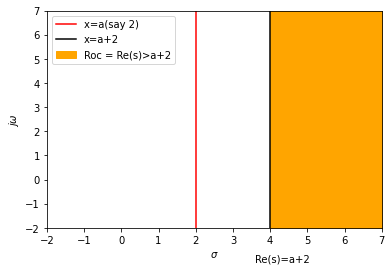
\includegraphics[width =\columnwidth ]{q3_gate}
\end{figure}








\end{document}